  \documentclass[twocolumn,onesided,9pt]{article}

\usepackage{./Task32FlyerLatexStyle/Task32Flyer}
\usepackage{todonotes}

%% -----------------------------------
%% Document information
%% -----------------------------------
\def\pubdate{DRAFT 22 April 2020}
\title{Using Ground-Based Vertically-Profiling Wind Lidar For Wind Resource Assessment in 2020}
\shorttitle{Vertically-Profiling Wind Lidar For Wind Resource Assessment in 2020}
\DOI{10.5281/zenodo.xxxxxx}
\addbibresource{bibliography.bib}

\newcommand{\conceptDOI}{http://dx.doi.org/xxx.xxxx}

%% ===================================
%% Document - specific commands
%% ===================================
%\usepackage[export]{adjustbox}
\newcommand{\IEARP}{\emph{RP-15}}
\newcommand{\IEARPn}[1]{\IEARP\ \emph{RP #1}}
\newcommand{\IEARPnote}[1]{\IEARP\ \emph{Note #1}}
\newcommand{\IEARPndetails}[2]{\IEARP,\ \emph{RP #1}:\ `#2'}
\newcommand{\IEARPnotedetails}[2]{\IEARP,\ \emph{Note #1}:\ `#2'}

%% ===================================
%% Document starts
%% ===================================
\begin{document}
	
	%% -----------------------------------
	%% Title
	%% -----------------------------------
\maketitle
\thispagestyle{cover}
	
%% -----------------------------------
%% Introductory text
%% -----------------------------------
{\Large\noindent%
IEA Wind published recommended practices on ground-based remote sensing for wind resource assessment in 2013. But what are the relevant standards for wind lidar for this use case in 2020?
}
\vskip 6pt
	
In this status update we give our perspective on best practices when deploying vertically-profiling wind lidar for wind resource assessments in 2020.
	
%% -----------------------------------
%% Why
%% -----------------------------------
\section*{Why an update?}
In 2013 IEA Wind Task 32 and Task 11 published "Recommended Practices ground-based remote sensing for wind resource assessment" \cite{RP15_2013}, or \IEARP. It was published in response to a need from the wind energy community for a document that described repeatable good practice in measurements with active remote sensing devices (RSDs), including lidar and sodar.
	
Since 2013, IEA Wind Task 32 and others have developed and codified new understanding of how best to use wind lidar. As a result, it is no longer clear what documents a user should turn to for guidance.
	
\subsection*{Our goal}
The goal of this update is the same as \IEARP, but is focused specifically on wind lidar:
	
\begin{shadequote}[r]{RP-15 (2013)}
... to document the steps required to collect high-quality, well-documented [wind lidar] data for use in wind resource assessments on land.
	\end{shadequote}
	
\subsection*{Our use case}
The use case considered here is the same as \IEARP, but limited to wind lidar:

\begin{shadequote}[r]{RP-15 (2013)}
... ground-based, fixed scan geometry, vertically-profiling wind remote sensing using [lidar] ... for the resource assessment phase of an on-shore wind farm development.''
\end{shadequote}
	
	
%% -----------------------------------
%% Relevant documents
%% -----------------------------------

\section*{What documents are relevant?}
	
The \href{https://github.com/IEA-Wind-Task-32/RP15-Ground-Based-Remote-Sensing-for-Wind-Resource-Assessment/releases/tag/1.0}{2013 IEA Wind Recommended Practices document} provided specific guidance as ``Recommended Practices'' (e.g., \IEARPn{1}) and informative notes (e.g. \IEARPnote{1}) about how to use remote sensing. These covered many different aspects of the remote sensing lifecycle. The \emph{RP}s were not always based on evidence, and so the document was called a ``recommended practices'', not a standard.
	
% \begin{figure}[h]
	% 	\centering
	% 	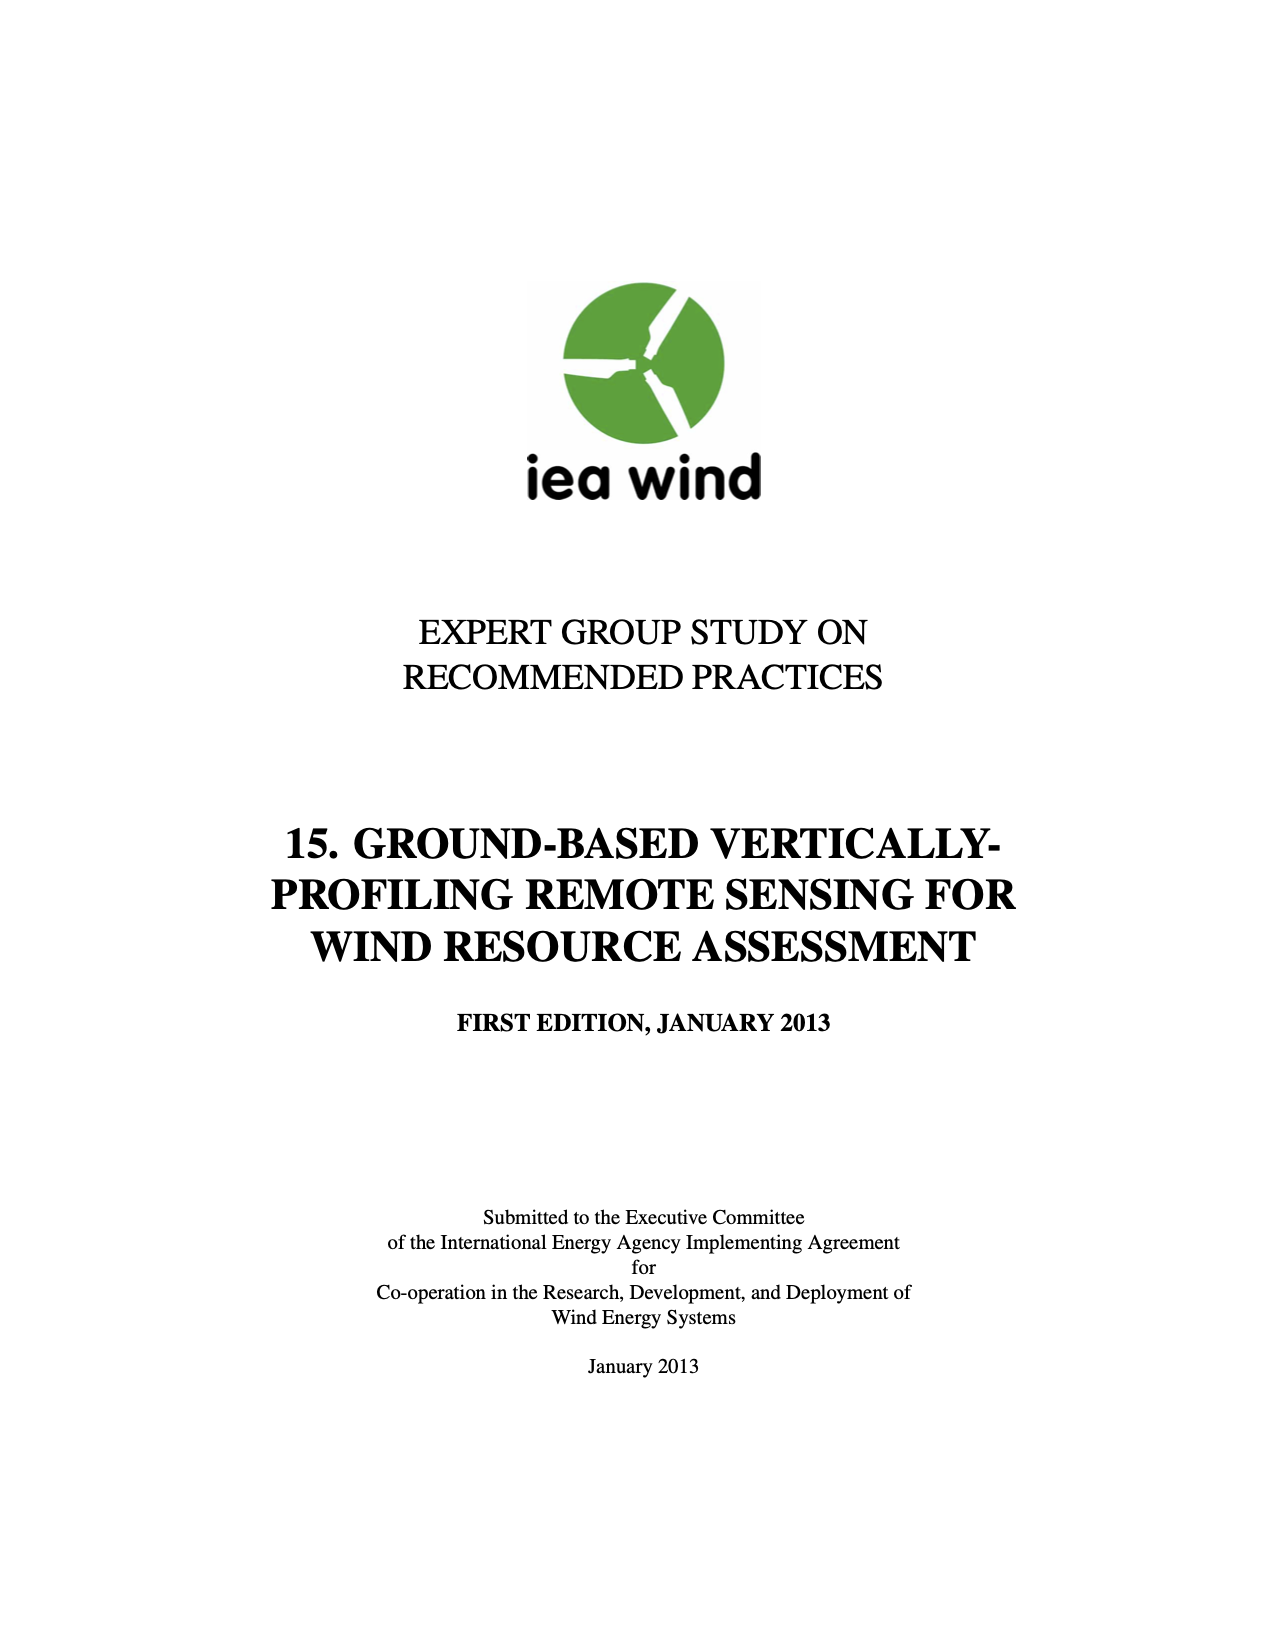
\includegraphics[width=0.9\linewidth, frame]{graphics/RP2013.png}
	% 	\caption{The 2013 Recommended Practices}
	% 	\label{fig:RP15_2013}
	% \end{figure}

In 2017 the International Electrotechnical Committee published a new edition of the IEC 61400-12-1 standard for power performance testing of wind turbines \citep[IEC 61400-12-1 (2017), ][]{IEC_61400_12_1_2017}. The IEC 61400-12-1 standard has traditionally been used as a \emph{de facto} standard for the measurements required for a wind resource assessment. It includes Annex L on the use of remote sensing for wind measurements. As a result, some groups also consider this standard to be applicable to the use case we consider here.

\todo[inline]{Are there other documents we should consider / mention, e.g. TR6?}

	%% -----------------------------------
	%% What to do in 2020
	%% -----------------------------------
	\section*{What to do in 2020}
	The following section identifies the documents that are applicable to the lifecycle of a wind lidar deployment:
	
	\begin{itemize}
		\item Characterising wind lidar
		\item Installing wind lidar
		\item Operating wind lidar
		\item Lidar data analysis
		\item Verification of wind lidar.
	\end{itemize}
	
	%% -----------------------------------
	%% Characterising RSD (RP1)
	%% -----------------------------------

	\subsection*{Characterising remote sensing devices}
	It is important that the technology used in the lidar is well characterized for future reference. This is covered in \IEARPndetails{1}{Documentation of RSD characteristics}.
	 
	%% -----------------------------------
	%% Installing RSD (RP2-16)
	%% -----------------------------------

	\subsection*{Installing wind lidar}
	\subsubsection*{Training}
	Users are encouraged to take specialist training on the wind lidar before deploying the device. This is covered in \IEARPndetails{2}{Training of workers}.

	\subsubsection*{Site selection}
	Current generations of wind lidar and their data processing tools are usually able to deal with obstructions or small-scale inhomogeneity (i.e. smaller than the scanning volume of the lidar). Therefore it is not necessary to completely avoid tower or structure wakes or deployments where part of the lidar scan pattern is obstructed. Instead, measurements that might include tower or structure wakes, or where the measurement beam is partly obstructed, should be carried out according to the manufacturer's recommendations. (This replaces \IEARPn{6 c and d} from 2013.)
		
	In \IEARP\ it was recommended to deploy lidar in an area where terrain-induced flow inhomogeneity in the measurement volume is minimal (\IEARPndetails{3}{Deployment in complex flow environments}). This was to minimize the potential differences between a wind lidar measurement (which are volumetric), and data from a cup anemometer, wind vane, or other point measurements.
	
	There are now many commercially-available tools and services that make it possible to use data from wind lidars deployed in more inhomogeneous flows (often called `complex flows') than was considered appropriate in 2013. Therefore, the siting constraint created by \IEARPndetails{3}{Deployment in complex flow environments} no longer applies.
	
	Instead, we recommend that the data from a lidar operating in complex flow conditions should be treated with the complex flow in mind. This may include different ways of processing the lidar line-of-sight data, statistical models, flow models, or other approaches. We further recommend following the recommendations of the lidar vendor or experienced consulting engineers about the use of wind lidars in complex terrain.
	
	Note: The challenge for the wind energy industry in 2020 is to identify the flow conditions where such tools may be required, and the potential benefit from using them. This is an active research topic.

	\todo[inline]{Not sure about the above section. Also feel like we could use this as a chance to raise this as an important research problem.}
	
	\subsubsection*{Transport}
	Any piece of wind measurement equipment should be handled with care during transport. This is covered in \IEARPndetails{4}{Reusable protective packaging for RSD transport} and \IEARPndetails{5}{Installation of shock detectors on the RSD}.
	
	\subsubsection*{Site preparation}
	Recommendations for site preparation to help ensure a successful deployment are given in \IEARPn{6 a and b}.
		
	\subsubsection*{Lidar orientation}
	It is important to document the lidar's compass orientation. Appropriate recommended practices are described in \IEARPndetails{7}{Device alignment}.
	
	\subsubsection*{Tilt and roll}
	It is important to monitor the lidar's tilt and roll with respect to  vertical. This may be required for data analysis or to monitor the lidar's stability. Appropriate recommended practices are given in \IEARPndetails{8}{Device leveling} and \IEARPndetails{9}{Tilt sensors on the RSD}.
	
	\subsubsection*{Time synchronization}
	Comparing data from multiple sources (for example, a wind lidar and a traditional tower) requires that the different data be sychronized. Appropriate recommended practices are given in \IEARPndetails{10}{Time sychronization}.
	
	\subsubsection*{Power supply}
	It is recommended to carefully choose a mature and proven power supply option for any site without grid-supplied electricity. Appropriate recommended practices are given in \IEARPndetails{11}{Design of remote power systems}.
	
	Remote power systems that have any kind of on-site fuel require special care and preparation. Appropriate recommended practices are given in \IEARPndetails{12}{Fuelled remote power systems}.
	
	\subsubsection*{Protection from interference}
	Like any unattended equipment, care should be taken to protect a ground-based lidar from interference. This is covered in \IEARPndetails{13}{Protection from interference}.
	
	\subsubsection*{Safety signs and interlocks}
	The need for safe operation and signage is covered in \IEARPndetails{14}{safety signs, interlocks and operation}.
	
	\subsubsection*{Function check}
	It is important to check that the lidar is working properly before being left unattended. A checklist was suggested in \IEARPndetails{15}{Function checklist}. These checks are still useful, but now might be implemented as part of automated tests by the lidar.

	\subsubsection*{Installation report}
	An installation report can add value to the final data set that is used in the wind resource assessment by reducing uncertainty. This is described in \IEARPndetails{16}{Installation report}.
	
	The content of the installation report should be checked with other data users.
	
	\subsection*{Operating wind lidar}
	\subsubsection*{Communications}
	\IEARP gives recommendations for how to provide remote access to a wind lidar (\IEARPndetails{17}{Remote access to the RSD}).
	
	\subsubsection*{Sensitivity to ambient conditions}
	In 2013, wind lidar were still relatively new devices and there was a lack of consensus about their behaviour in different weather conditions. \IEARPn{18 and 19} recommended that measures should be taken to document and if possible, mitigate the effects of ambient conditions on the RSD. Since then, tests for the sensitivity of lidar and other remote sensing devices have been introduced as part of IEC 61400-12-1 (2017). These form part of the lidar uncertainty classification. Therefore, \IEARPn{18 and 19} are no longer valid.
	
	If they need such information, lidar users can request an uncertainty classification document that meets the needs of IEC 61400-12-1 (2017) from the lidar vendor or through a third party.
	
	\subsubsection*{Local weather conditions}
	It is important to collect weather data at or near the lidar. These should measure any parameters that have been found to be important using the  sensitivity assessment approach given in IEC 61400-12-1 (2017).
		
	\subsubsection*{Servicing and maintenance}
	Like all wind measurement devices, wind lidar may require maintenance from time to time.
	
	Appropriate recommendations about how wind lidar users and suppliers should work together to ensure reliability and repeatability are provided in \IEARPndetails{23}{Recommended service intervals}.
	
	\subsubsection*{Operation and maintenance log}
	Users should keep a log of all use and maintenance of the wind lidar. This is described in \IEARPndetails{24}{Operation and maintenance log}.
	%
	%% -----------------------------------
	%% Remote sensing data analysis (RP 25-29)
	%% -----------------------------------
	\subsection*{Remote sensing data analysis}
	
	\subsubsection*{Wind speed and vector}
	The wind lidar should save data at different steps in the internal data processing. This may include the following:
	
	\begin{enumerate}
		\item Line-of-sight data, as described in \IEARPndetails{25}{Line-of-sight wind velocity}.
		\item Reconstructed wind data, as described in \IEARPndetails{26}{Instantaneous wind vector}. \IEARPn{26 c} is no longer required as the information needed by a user can be derived from the data.
		\item Tim-averaged wind vector, as described in \IEARPndetails{27}{Time-averaged wind vector}.
\end{enumerate}

\subsubsection*{Turbulence intensity}
In 2013 when the IEA RP-15 was published it was not clear if wind turbulence values derived from wind lidar data could be directly compared to turbulence data from cup anemometers.
	%
Since then, there has been much research into the ability of wind lidar to measure wind turbulence \citep[see e.g.,][]{sathe_2016_a, clifton_2018_a}. The current consensus in the wind lidar community is that the wind turbulence derived by a wind lidar is not the same as measured by a cup anemometer, but there may be ways to adjust the two values so that they agree.
	%
For those reasons, \IEARPndetails{28}{Derivation of turbulence intensity} is no longer applicable.

We suggest that turbulence data derived from wind lidar may be used if there is an appropriate validation of the methods against a reference device. The validation should be carried out in comparable terrain and comparable atmospheric conditions.

Because this turbulence data could be derived by many different methods (e.g., by the lidar as part of the measurements, by the lidar's post-processing software, by third-party software, or other methods), thought should be given to developing an auditable data processing chain.

\subsubsection*{Extreme gusts}
Gust data from wind lidar can be used if they have been validated against measurements from a cup anemometer. This should follow the same validation processes as used for wind speed and wind turbulence data.

%% -----------------------------------
%% Verification of remote sensing devices (RP 30 - 41)
%% -----------------------------------
	%
\subsection*{Verification of remote sensing devices}
\todo[inline]{Verification or validation? Let's align with IEC?}
\IEARP\ included recommendations about how to test the performance of a remote sensing device, quantify it, estimate uncertainty, and how to document it. These RPs (\IEARPn{30 -- 40}) may still be helpful for users who are interested in carrying out performance checks on their own wind lidar. However, the methods described in \IEARP\ do not provide the information necessary for a wind resource assessment.

We recommend that a wind lidar being used as part of the financing package for a wind energy facility undergo an uncertainty classification according to the IEC 61400-12-1 (2017) standard \cite{IEC_61400_12_1_2017}.
		
\section*{Future developments}
The state of the art in wind lidar measurements will continue to develop, and there will be new standards published. We are aware of the following activities that may be relevant:
	
	\begin{itemize}
		\item An IEA Wind Task 32 working group on the use of wind lidar in complex terrain is carrying out a group study on several different tools to support the use of wind lidar in complex terrain. Results are expected in 2021 and may lead to the publication of guidelines for that use case.
		
		\item The effectiveness of several tools to adjust wind lidar turbulence data will be investigated by the Consortium for the Advancement of Remote Sensing (CFARS, \href{http:\\www.cfars.org}{www.cfars.org)} in 2020.
		
		\item The IEC is also in the process of updating the body of standards relating to wind energy (the IEC 61400 series). During 2020-2022 new standards are expected on ...

		\todo[inline]{50-3 etc.}
				
		\item ...
		
	\end{itemize}
	
	As a result of these developments, we anticipate revising this document again during the period 2021-2023 to reflect new developments. Readers are encouraged to check \href{\conceptDOI}{\conceptDOI} for revisions.
	
	\section*{Summary}
	Many of the 2013 IEA Wind Recommended Practice 15 on Ground-Based Vertically-Profiling Remote Sensing For Wind Resource Assessment are still relevant in 2020, particularly in relation to general good practice when deploying, operating, and maintaining wind lidar.
	
	Since 2013 the wind energy community has gathered a huge amount of experience in using wind lidar data. Therefore in 2020 we recommend that turbulence and gust data derived from wind lidar measurements can be used, if verification studies can be provided. 
	
	Almost all of the verification approaches suggested in the 2013 \IEARP\ have been superseded by the publication in 2017 of the IEC 61400-12-1 Standard for power performance measurements \cite{IEC_61400_12_1_2017}. It is our expectation that the development of a new family of IEC standards for instrumentation and measurements in the 2020's may in turn deprecate the 2017 edition of the IEC 61400-12-1 standard.
	
%% -----------------------------------
%% Feedback
%% -----------------------------------
	
\section*{Your feedback and comments}
Feedback about the 2013 Recommended Practices document should be made via the \href{https://github.com/IEA-Wind-Task-32/RP15-Ground-Based-Remote-Sensing-for-Wind-Resource-Assessment/issues}{GitHub repository}.

Feedback about this status update should be directed to the \href{https://github.com/IEA-Wind-Task-32/RP15-Ground-Based-Remote-Sensing-for-Wind-Resource-Assessment}{Task 32 Operating agents}.

	
    %% -----------------------------------
    %% References
    %% -----------------------------------
    %\subsection*{References}
    % bibliography
    \label{sec:References}
    \addcontentsline{toc}{section}{References}
    {\small
    \printbibliography
    }
    \vspace*{\fill}


    %% -----------------------------------
    %% Outlined block of smaller text
    %% -----------------------------------
\begin{tcolorbox}[width=1.0\columnwidth,
	boxsep=0pt,
	left=3pt,
	right=3pt,
	top=3pt,
	arc=0pt,
	boxrule=0.5pt,
	toprule=0.5pt,
	colback=white,
	coltext=TextGrey
	]
{%
%% -----------------------------------
%% IEA WIND AND TASK 32
%% -----------------------------------
\noindent%
\footnotesize%
\begin{center}%
\vspace{-2mm}
\begin{tabular}{m{0.3\columnwidth}m{0.6\columnwidth}}
\multicolumn{2}{m{\dimexpr0.9\columnwidth+2\tabcolsep\relax}}{This document was self published by IEA Wind Task 32.}\\
% IEA Wind * DO NOT EDIT THIS TEXT *

\includegraphics[height=2cm]{graphics/IEAWind_logo.jpg}
&
The International Energy Agency is an autonomous organisation which works to ensure reliable, affordable and clean energy for its 30 member countries and beyond. \href{https://community.ieawind.org}{The IEA Wind Technology Collaboration Programme} supports the work of 38 independent, international groups of experts that enable governments and industries from around the world to lead programmes and projects on a wide range of energy technologies and related issues.
\\
% Task 32 * DO NOT EDIT THIS TEXT *
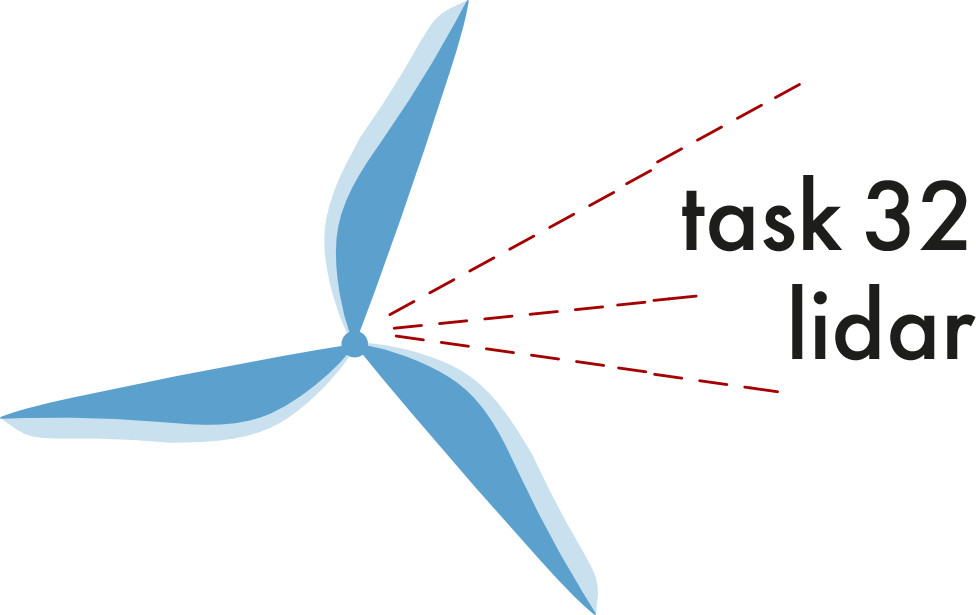
\includegraphics[height=1.5cm]{graphics/Task32_logo.jpg} &
\href{https://community.ieawind.org/task32/home}{IEA Wind Task 32} exists to identify and mitigate the barriers to the deployment of wind lidar for wind energy applications.
\\
%% -----------------------------------
%% More information
%% -----------------------------------
\multicolumn{2}{m{\dimexpr0.9\columnwidth+2\tabcolsep\relax}}{
% N.B. do not add line breaks between the next items
%% -----------------------------------
%% Authors
%% -----------------------------------
\textbf{Author team:} %
Andrew Clifton (Task 32 Operating Agent, University of Stuttgart, Germany), %
xxx (org x), %
yyy (org y).
%% -----------------------------------
%% Reviewers
%% -----------------------------------
\textbf{Reviewers:} %
aaa (org x), %
bbb (org y).
%% -----------------------------------
%% Images
%% -----------------------------------
\textbf{Image credits:}
Banner, left to right: \href{https://unsplash.com/@alexkixa}{Alexandre Debiève on Unsplash}, \href{http://ifb.uni-stuttgart.de}{SWE U. Stuttgart}, \href{https://unsplash.com/@markusspiske}{Markus Spiske on Unsplash}.
} % end of more information
\end{tabular}
\end{center}
} % end of footnotesize
\end{tcolorbox} % end of tcolorbox
%% -----------------------------------
%% End of highlighted block
%% -----------------------------------
\vspace*{\fill}

\end{document}
